
%%% Local Variables: 
%%% mode: latex
%%% TeX-master: t
%%% End: 
\documentclass[twocolumn]{article}

% Packages
% \usepackage{fancyhdr}
\usepackage{amsmath}
\usepackage{amssymb}
\usepackage[margin=10mm]{geometry}
\usepackage{xcolor}
\usepackage{graphicx}



% Housekeeping
\pagestyle{empty}


\begin{document}
\section{Artificial Intelligence}
\label{sec:artif-intell}

%%% Ideas:
% There should be more than these note points. Add some when you do
% the second time reviewing.
\begin{itemize}
% \item Life is fucking awesome in the United Arab Emirates!
% \item Life is a bitch. Fuck it or leave it, choose one.
\item An \textbf{agent} is an entity that can perceive and act. This
  course is about designing rational agents. 
\item Rational behavior: doing the right thing. 
\item Environment Types: Fully observable; Deterministic; Episodic;
  Static, Discrete; Single-agent. The counter part: partially
  observable; stochastic; sequential; dynamic; continuous;
  multi-agent. 
\item An agent is anything that can be viewed as perceiving its
  environment through sensors and acting upon that environment through
  actuators.
\item Being rational means maximizing your \textbf{expected
    utility}. And a better title for this course would be
  \textbf{Computational Rationality}.
\item \textbf{Rational:} maximally achieving pre-defined goals.
\item \textbf{Rationality:} only concerns what decisions are made (not
  the thought process behind them)
\item \textbf{Utility:} Goals are expressed in the terms of the
  utility of outcomes. And CS188 thinks that being rational means
  maximizing your expected utility.
\item \textbf{Automation:} Applied AI involves many kinds of
  automation. Scheduling, route planning, medical diagnosis, web
  search engines, spam classifiers, automated help desks, fraud
  detection, product recommendations. ``Did any one of these remind
  you of subtopics and projects in Machine Learning?'' 
\item \textbf{Agent:} An agent is an entity that perceives and acts. A
  rational agent selects actions that maximize its \emph{expected}
  utility. 
\item Making decision, reasoning under Uncertainty, and their
  applications. 
\end{itemize}


\section{Problem Solving}
\label{sec:problem-solving}

\begin{itemize}
% \item Life is fucking awesome in the United Arab Emirates!
\item A search problem consists of 
  \begin{itemize}
  \item a state space
  \item a successor function (namely \textbf{update function} in data
    mining algorithm series, more namely \textbf{recursion} in
    bullshit technology.)
  \item a start state (\textbf{initial value}), goal test
    (\textbf{terminating value}) and path cost function (\textbf{we
      say weights in Graph Theory})
  \item Does any one of the above reminds you of \textbf{recursion}?
  \end{itemize}
\item Problems are often modelled as a state space, a set of states
  that a problem can be in. The set of states forms a graph where two
  states are \textbf{connected} if there is an operation that can be
  performed to transform the first state into the second.
\item A solution is a sequence of actions (a plan) which transforms
  the start state to a goal state.
\item \textbf{State space graph}: A mathematical representation of a
  search problem.
\item \textbf{Search Trees} 
  \begin{itemize}
  \item This is a ``what-if'' tree of plans and outcomes
  \item For most problems, we can never actually build the whole tree
  \end{itemize}
\item \textbf{General Tree Search} Frontier; Expansion; Exploration
  Strategy.
\item \textbf{States vs. Nodes} Nodes in state space graphs are
  problem states; Nodes in search trees are plans. {\color{red}The same problem
  state may be achieved by multiple search tree nodes.}
\item \textbf{Graph Search} Graph Search still  produces a search
  tree; Graph search is almost always better than tree search.
\item DFS graph search needs to store ``explored set'', which is
  $O(b^{m})$. However, \textbf{DFS is optimal} when the search tree is finite,
  all action costs are identical and all solutions have the same
  length. However limitating this may sound, there is an important
  class of problems that satisfies these conditions: the CSPs
  (constraint satisfaction problems). Maybe all the examples you
  thought about fall in this (rather common) category. 
\item The breadth first search and iterative deepening are
  conceptually and computationally the same. The only difference is
  the ``space'' (we call them \textbf{memory}) would be partially
  saved by iterative deepening search.
\item \textbf{Heuristics} estimate of how close a node is to a goal;
  Designed for a particular search problem. 
% \item Life is fucking awesome in the United Arab Emirates.
\item \textbf{A star search} Uniform-cost orders by \textbf{path cost}, or
  backward cost  $g(n)$; Best-first orders by \textbf{distance} to goal, or
  forward cost $h(n)$. A* Search orders by the sum:
  $f(n)=g(n)+h(n)$. The distance is an estimated one.
\item When A* terminates its search, it has, by definition, found a
  path whose actual cost is lower than the estimated cost of any path
  through any node on the frontier. But since those estimates are
  optimistic, A* can safely ignore those nodes.
\item In general, most natural admissible heuristics tend to be
  consistent, especially if from relaxed problems. 
% \item Something extra while reviewing online courses.
\item Types of agents: reflex agents, planning agents (optimal
  vs. complete planning).
\end{itemize}

\subsection{Uninformed Search}
\label{sec:uninformed-search}

\begin{itemize}
\item \textbf{State Space:} A state space is also an abstraction of
  the world. A successor function \textbf{models} how your world
  works (namely, evolves and response to your actions). 
\item \textbf{Search Problems:} They are just models, aka, no more
  than models in the mathematical sense.
\item \textbf{World State:} Includes every last detail of the
  environment. 
\item \textbf{Search State:} Keeps only the details needed for
  planning (namely, abstraction). Because only with abstraction can we
  solve problems smoothly.
\item \textbf{Search Trees:} For most problems, we can never actually
  build the whole tree. (So we \textbf{ignore} most of the tree.)
\item \textbf{Complete:} Guaranteed to find a solution if one exists?
  \textbf{Optimal:} Guaranteed to find the least cost path?
\item \textbf{DFS vs BFS:} When will one outperform the other?
\item \textbf{Uniform Cost Search:} Expand a cheapest node first. Thus
  fringe is a \textbf{priority queue}. (priority, cumulative cost,
  namely, add them up!) Therefore it's complete and optimal! But it
  explores options in every ``direction''. And this algorithm shows
  \textbf{no information} about goal location.
\item Search operates over \textbf{models} (namely, abstractions) of
  the world. Planning is all ``in simulation'', therefore your search
  is only as good as your model is.
\end{itemize}

\subsection{Informed Search}
\label{sec:informed-search}

\begin{itemize}
\item \textbf{Informed Search:} Inject information of where the goal
  might be. Key idea: Heuristics.
\item \textbf{Successor Function:} If I do this, what will
  happen, in my model.
\item \textbf{Search Heuristics:} Something tells you that whether you
  are getting close to the goal, or not. It's a function that
  \emph{estimates} how close a state is to a goal. It's designed for a
  particular search. Examples: Manhattan distance, euclidean
  distance. (They are not perfect, but they are \emph{at least}
  something.) 
\item \textbf{Greedy Search:} A common case: best-first takes you
  straight to the (wrong) goal.
\item \textbf{A* Search:} Revised. Combine both UCS and Greedy,
  namely, tortoise and rabbit. Uniform-cost orders by path cost, or
  backward cost. Greedy orders by goal proximity, or forward cost.
\item \textbf{A* Search:} Stop when you \textbf{dequeue} a goal from
  the fringe. Lesson: We need estimates to be less than actual costs.
\item \textbf{Admissibility:} Admissible (optimistic) heuristics slow
  down bad plans but never out-weight true costs. Inadmissible is just
  a fancy name for, \textbf{pessimistic}, it traps good plans on the
  fringe. 
\item A heuristic \textbf{h} is \textbf{admissible} (optimistic) if: 
  \begin{equation}
    \label{eq:1}
    0\leq h(n)\leq h^{*}(n)
  \end{equation}
  where $h^{*}(n)$ is a true cost to a nearest goal. Thus coming up
  with admissible heuristics is most of what's involved in using
  $A^{*}$ in practice. $A^{*}$ is not problem specific, but your
  heuristic is.
\item \textbf{Crating Admissible Heuristics:} Most of the work in
  solving hard search problems optimally is in coming up with
  admissible heuristics. Often, admissible heuristics are solutions to
  \textbf{relaxed problems}, where new actions are available.
\item \textbf{Graph Search:} For tree search, if it fails to detect
  repeated states can cause exponentially more work. Idea:
  \textbf{never expand} a state twice.
\item Important: (in python's idea) store the closed set as a set, not
  a list. In Lisp's concept, make it a hash table (it is verified,
  just use hash table in Lisp).
\item \textbf{Consistency of Heuristics:} real cost should be larger
  or equal than cost implied by heuristic. (Namely, please be
  \textbf{Conservative}, aka guess ``smally'' rather than
  ``biggerly''.) Implication: $f$ value along a path never decreases. 
\item \textbf{Optimality:} For tree search, requires heuristic
  admissible; for graph search, requires consistent. And consistency
  implies admissibility.
\item \textbf{Heuristics:} The design of this number (function) is
  key, often use \textbf{relaxed problems}.
\end{itemize}

\subsection{Constraint Satisfaction Problems}
\label{sec:constr-satisf-probl}

\begin{itemize}
% \item Life is fucking awesome in UAE!
\item \textbf{Search:} a single agent, deterministic actions, fully
  observed state, discrete state space.
\item \textbf{Planning:} a sequence of actions. The \textbf{path} to
  the goal is the important thing.
\item \textbf{Identification:} assignments to variables. The goal
  itself is important, not the path.
\item \textbf{CSP:} a special subset of search problems. State is
  defined by \textbf{variable $X_{i}$} with values from a domain $D$
  (sometimes $D$ depends on $i$). Goal test is a set of constraints
  specifying allowable combinations of values for subsets of
  variables. 
\item CSP allows useful general-purpose algorithms with more power
  than standard search algorithms. (Namely, add more ``rules'', walk
  through (traverse) less paths.)
\item \textbf{CSP Varieties:} Discrete variables; continuous
  variables.
\item \textbf{Varieties of Constraints:} Unary; Binary; Higher-order
  constraints. Or Preferences (soft constraints).
\item \textbf{Backtrack Search:} The basic uninformed algorithm for
  solving CSPs. Namely, recursion. One variable at a time; check
  constraints as you go (Online shit? Incremental goal test). So
  backtracking is equal to DFS add variable ordering and add
  fail-on-violation. 
\item \textbf{Improve Backtracking:} Ordering; Filtering; Structure. 
\item \textbf{Filtering:} Keep track of domains for unassigned
  variables and cross off bad options. Namely, build a mathematical
  filter. Namely, ask (cond, else) when doing forward checking.
\item \textbf{Forward Checking:} Enforcing consistency of arcs
  pointing to each new assignment. 
\item \textbf{Arc Consistency:} It still runs inside a backtrack
  search.
\item \textbf{Ordering:} Minimum Remaining Values. Variable ordering,
  \textbf{always} choose the variable with the \textbf{fewest} legal
  left values in its domain, given a choice of variables.
\item What the hell is CSP? Variables; Domains;
  Constraints---Implicit, Explicit, Unary/Binary/N-ary. Goals: find
  any solution; find all; find best, etc.
\item \textbf{K-Consistency:} For each k nodes, any consistent
  assignment to $k-1$ can be extended to the $k^{th}$ node.
\item Suppose a graph of $n$ variables can be broken into subproblems
  of only $c$ variables. Example: $n=80, d=2, c=20$. But this ``crap''
  is somehow impractical. 
\item \textbf{Tree-Structured CSPS:} Theorem, if the constraint graph
  has no loops, the CSP can be solved in $O(nd^{2})$ time. For general
  CSPs, worst case is $O(d^{n})$. This also applies to probabilistic
  reasoning: an example of the relation between syntactic restrictions
  and the complexity of reasoning.
\item \textbf{Nearly Tree-Structured CSPs:} Cutset conditioning:
  instantiate (in all ways) a set of variables such that the remaining
  constraint graph is a \textbf{tree}.
\item \emph{Sorry this is in ai class, everything is hard.---CS188}
\item \textbf{Tree Decomposition:} Create a tree-structured graph of
  mega-variables. Each mega-variables encodes part of the original
  CSP. 
\item CSPs are a special kind of search problems where states are
  partial assignments and goal test is defined by constraints. The
  basic solution is backtrack search.
\item \textbf{Local Search:} (yet another fancy name of EM algorithm.)
  It improves a single option until you can't make it
  better. (\textbf{No fringe!}) 
\item Generally local search is much faster and more memory
  efficient. But it is also \textbf{incomplete and suboptimal}.
\item \textbf{Hill Climbing:} Simple general idea---Start wherever,
  repeat: move to the best neighboring state; if no neighbors better
  than current, quit.
\item \textbf{Simulated Annealing:} Idea, escape local maxima by
  allowing downhill moves.
\item The more downhill steps you need to escape a local optimum, the
  less likely you are to ever make them all in a row. Therefore people
  think hard about ridge operators which let you jump around the space
  in better ways.
\item \textbf{Genetic Algorithms:} It uses a natural selection
  metaphor---keep best N hypotheses at each step based on a fitness
  function; Also have pairwise crossover operators, with optional
  mutation to give variety. 
\end{itemize}

\subsection{Adversarial Search}
\label{sec:adversarial-search}

\begin{itemize}
% \item Life is fucking awesome in the United Arab Emirates!
\item \textbf{Meaning:} How to decide how to act, when there is an
  adversary in ``your world (model, abstraction, etc.)''.
\item Monte Carlo methods are just a fancy name for
  \textbf{randomized} methods.
\item \textbf{Pacman:} Behavior from \textbf{Computation}.
\item \textbf{Axes:} Deterministic or stochastic? One, two or more
  players? Zero sum? Perfect information (can you see the state)?
\item For this course, we want algorithms for calculating a
  \textbf{strategy (policy)} which recommends a \textbf{move} from
  each state.
\item Different from search: we do not \textbf{control} our
  opponent. We need to give out \textbf{policies}.
\item One possible formalization is: States, Players, Actions,
  Transition Function $S\times A\rightarrow S$, Terminal Test $S\rightarrow
  \{t,f\}$, Terminal Utilities $S\times P\rightarrow R$.
\item Players usually take turns; Actions may depend on player/state;
  Terminal utilities tells us how much it's worth to \textbf{each of
    the players}. 
\item \textbf{Zero-Sum Games:} Let us think of a single value that one
  maximizes and the other minimizes.
\item \textbf{General Games:} Agents have independent
  utilities. Cooperation, indifference, competition, and more are all
  possible. 
\item  \textbf{Value} of a state: The \textbf{best} achievable outcome
  (utility) from that state.
\item \textbf{Minimax Values:} States Under Opponent's Control:
  $V(s')= min~V(s)$ States Under Agent's Control: \textbf{Maximize}
  out of all possible ``worst'' results your \textbf{opponent}
  offers. In choosing universities and advisors, pick out the
  ``tallest'' guy from the ``small man''. 
\item In other words, life is much much worse when there is an (or
  more than one) adversary. I want the ``global maximum'', but the
  adversary just \textbf{won't let it happen}.
\item \textbf{Minimax Search:} A state-space search tree; players
  alternate turns; compute each node's \textbf{minimax value}, namely
  the best achievable utility against a rational (optimal) adversary.
\item Ask this question to yourself: do we \textbf{really} need to
  explore the whole tree?
\item \textbf{Resource Limits:} In realistic games, cannot search to
  leaves. Solution: \textbf{Depth-Limited Search}. Search only to a
  limited depth in the tree, and replace terminal utilities with an
  evaluation function for non-terminal positions.
\item \textbf{Depth Matters:} An important example of the tradeoff
  between complexity of features and complexity of computation.
\item \textbf{Evaluation Functions:} In practice, typically weighted
  linear sum of features. 
\item \textbf{Game Tree Pruning:} Look at the trees that do not have
  to be minimized. 
\item \textbf{Alpha-Beta Pruning:} Key idea it symmetric. To sum up,
  it's already \textbf{bad enough} that it won't be played. $\alpha$
  MAX's best option on the path to root. $\beta$ MIN's best option on
  path to root. Tip: You have to be right for the children of the
  route. Therefore good child ordering improves effectiveness of
  pruning. 
\end{itemize}

\section{Uncertain Knowledge and Reasoning}
\label{sec:uncert-knowl-reas}



\subsection{Expectimax and Utilities}
\label{sec:expectimax-utilities}

\begin{itemize}
\item Uncertain outcomes controlled by \textbf{chance}, not an
  adversary!
\item Values should now reflect average-case (expectimax) outcomes,
  not worst-case (minimax) outcomes. (Explicit randomness,
  Unpredicable opponents, Actions can fail).
\item \textbf{Expectimax search:} compute the average score under
  optimal play. Key idea: Calculate their \textbf{expected
    utilities}. 
\item For average-case expectimax reasoning, we need
  \textbf{magnitudes} to be meaningful. Not only order matters,
  magnitudes as well.
\item As we get more evidence, probabilities may change.
\item \textbf{Random variable} represents an event whose outcome is
  unknown.
\item \textbf{Probability distribution} is an assignment of
  \textbf{weights} to outcomes. Note, in functional programming, we
  can also say that it's a \textbf{mapping} of weights to outcomes.
\item The \textbf{expected value} of a function of a random variable
  is the \textbf{average}, weighted by the probability distribution
  over outcomes.
\item Having a probabilistic belief about another agent's action
  \textbf{does not} mean that the agent is flipping any coins!
\item Based on \textbf{how we think} the world works, what computation
  we should do. Are our opponents adversarial or by chance?
\item \textbf{Minimax} generalization:
  \begin{itemize}
  \item Terminals have utility tuples (namely, lists)
  \item Node values are also utility tuples
  \item Each player maximizes its own component
  \item Can give rise to \textbf{cooperation} and \textbf{competition}
    dynamically. 
  \end{itemize}
\item \textbf{Vampire Bunnies}
\item {\color{red} Worst case reasoning only works to the extent that
    your model is sufficiently simple.} Namely, \textbf{minimax} is
  just a \textbf{binary} ``crap'', though the world can be
  ``simulated'' based on asking \textbf{yes or nos}, it is still too
  young too simple, sometimes naive, naive! ``Yo you may be hit by a
  METEOR!!'' 
\item Tip: A rational agent should choose the action that maximizes
  its expected utility, \textbf{given its knowledge}.
\item \textbf{Utilities} are functions from outcomes (states of the
  world) to real numbers that describe an \textbf{agent's
    preferences}.
\item We hard-wire utilities and let behaviors emerge. The search
  procedure should do that for us. Behavior is complicated and
  \textbf{context} dependent.
\item Utilities can also be regarded as a reflection of
  \textbf{uncertain outcomes}. But win or lose, you play it.
\item An agent with \textbf{intransitive preferences} can be induced
  to give away all of its money. (Loop forever.)
\item Utility scales: normalized utilities, micromorts,
  quality-adjusted life years.
\item People would pay to reduce their risks.
\end{itemize}

\subsection{Markov Decision Processes}
\label{sec:mark-decis-proc}

\begin{itemize}
\item \textbf{MDP} A way of formalizing the idea of non-deterministic
  search, which is the search when your actions' outcomes are
  \textbf{uncertain}. 
\item \textbf{Noisy Movement} actions do not always go as planned.
\item An MDP is defined by: a set of states, a set of actions, a
  transition function, a reward function, a start state, and maybe a
  terminal state. Therefore, one way to solve the MDPs is with
  expectimax search. Namely, it's yet another \textbf{fancy search},
  but our \textbf{testing goal} has changed.
\item ``Markov'' means action outcomes depend only on the current
  state (namely, to simplify the calculation, we \textbf{do need to}
  make some assumptions.) This is just like search, where the
  \textbf{successor function} could only depend on the current state
  (not the history). Well, if you do want to depend on the history,
  GIFF more powerful computers and be a master of, you named it,
  \textbf{statistics and matrix}.
\item In deterministic single-agent search problems, we wanted an
  optimal plan, or sequence of actions, from start to a
  goal. (Actually same ``greedy ideas'' in non-deterministic problems,
  but in situations like this, we are forced to enjoy the
  \textbf{uncertainty}, which comes from, well, you named it, mother
  nature or rather, quantum mechanics.)
\item An optimal \textbf{policy} is one that maximizes expected
  utility \textbf{if followed}. When we say if, you know we are
  talking about the fucking \textbf{uncertainty}.
\item An \textbf{explicit} policy defines a reflex agent. 
\item \textbf{Reflex} an action that is performed as a response to a
  stimulus and without conscious thought. 
\item Expectimax did \textbf{not} compute entire policies, solutions,
  ideas, paths whatsoever. It computed the action for a single state
  only. But \textbf{IT WORKS}.
\item What \textbf{Markov} did is just to remove the redundancy so
  that we can use \textbf{minimal} information to \textbf{render} the
  things down.
\item \textbf{Your models are never going to be perfect.}
\item Each MDP state projects an expectimax-like search tree.
\item \textbf{Utilities of Sequences} Ask questions: more or less; now
  or later (mind the \textbf{discounting}). 
\item \textbf{Discounting} values of rewards (may and usually so)
  decay exponentially. It helps our algorithms \textbf{converge}!!!
\item \textbf{Infinite Utilities} Finite horizon, discounting or
  absorbing state (like ``overheated'' for racing). In general we will
  have \textbf{discounts}.
\item \textbf{Policy} Mapping from actions to states. \textbf{Utility}
  sum of (discounted) rewards.
\item \textbf{Values of States} fundamental operation: compute the
  (\textbf{expectimax}) value of a state. 
  \begin{itemize}
  \item Expected utility under optimal action.
  \item Average sum of (discounted) rewards.
  \item This is \textbf{just} what expectimax computed.
  \end{itemize}
\item Recursive definition of values:
  \begin{itemize}
  \item $V^{*}(s)={\displaystyle\max_{a}}Q^{*}(s,a)$
  \item The value of a state is the \textbf{max} over all the
    \textbf{actions} available to you.
  \item $Q^{*}(s,a)=\sum_{s'}T(s,a,s')[R(s,a,s')+\gamma V^{*}(s')]$
  \item We are going to get a reward in the next time step, and a
    \textbf{future} reward. They are going to be \textbf{weighted} by
    the \textbf{relative probabilities} that come from our
    \textbf{transition function}. Mind the future shit, so we need to
    add a \textbf{discount} on the future, because it's not what we
    get\@ NOW.
  \end{itemize}
\item States are repeated. Tree goes on forever. Note: deep parts of
  the tree eventually \textbf{does not} matter if $\gamma < 1$.
\item \textbf{Time-Limited Values} $V_{k}(s)$ is the \textbf{optimal}
  value of $s$ if the game ends in $k$ more time steps. Equivalently,
  it's what a \textbf{depth-k} expectimax would give from s. (Namely,
  life is short, PLEASE do not loop/recur forever, please\ldots)
\item Because we are just truncating, we are just ending the game---we
  \textbf{do not} need an evaluation function. Because \textbf{IT JUST
  STOPS}.
\item So it is a \textbf{trade-off} of how many states you have, how
  connected they are and how deeply you want to go into the tree.
\item Basic idea: approximations get refined towards optimal
  values. (When we say refine, we can also say, you guessed it,
  \textbf{filtering}.) 
\item \textbf{Convergence}
  \begin{itemize}
  \item If the tree has maximum depth M, then $V_{M}$ holds the actual
    untruncated values. \textbf{I have done the EM search} and any
    further iteration/recursion will do nothing (Namely, their
    \textbf{reward}, return, gains, utilities are considered,
    regarded, or set $0$, so it's ``mathematically'' dead, then we do
    \textbf{not} need to, you name it, do calculations \textbf{any
      more}). 
  \item If the discount is \textbf{less than} 1.
  \item The last layer is at best all $R_{\max}$.
  \item The last layer is at worst $R_{\min}$.
  \item But everything is \textbf{discounted} by $\gamma^{k}$ that far
    out. 
  \item So $V_{k}$ and $V_{k+1}$ are \textbf{at most} $\gamma^{k} \max
    |R|$ different.
  \item So as $k$ increases, the values converge because the
    \textbf{differences} are \textbf{smaller than smaller}. After all
    these ``smalling'' processes, it will die, or at least looks like
    ``dead''. That word means there is \textbf{no significant} further
    growth. 
  \end{itemize}
\end{itemize}

\subsection{Markov Decision Processes Continued}
\label{sec:mark-decis-proc-1}

\begin{itemize}
\item Oh! That's their probability of landing a $s'$.
\item \textbf{Policy} A map (surely it's with Python and Lisp) of
  states to actions.
\item Your transition function tells you what the \textbf{likelihoods}
  are. 
\item {\color{red} \textbf{Rewards} are instantaneous and \textbf{values} are
    accumulative.} It's an very important distinction. 
\item \textbf{How to be optimal:} Take correct first action; Keep
  being optimal. It's just some kind of recursive procedures, or some
  ``iterative dynamic programming''. Holy Jesus Lord, \textbf{they are
  actually fuckingly the same thing, will you be able to understand}?
  This of course is in terms of \textbf{implementation}. And isn't
  this concept called ``greedy'' in algorithm book?
\item Bellman equations \textbf{characterize} the optimal values; the
  \textbf{fuck yourself} algorithm ``computes'' them. Because of this,
  there is now a \textbf{real recursion}. It bottoms out at $0$. And
  suddenly we have a notion of times-attached.
\item Expectimax trees max over all actions to compute the
  \textbf{optimal} values.
\item Turn recursive Bellman equations into \textbf{updates}. Namely,
  it's just the fucking value iteration.
\item Without the maxes, the Bellman equations are just a
  \textbf{linear system}.
\item $\pi^{*}(s)={\displaystyle argmax_{a}}\Sigma
  T(s,a,s')[R(s,a,s')+\gamma V^{*}(s')]$ This is called \textbf{policy
  extraction}, since it gets the policy implied by the values. This is
  also called \textbf{reconstruct}.
\item $\pi^{*}(s)=argmax_{a}Q(s,a)$ Computing actions from
  \textbf{Q-Values} is completely trivial. And it is much easier to
  select from q-values than values.
\item What value iteration does, is essentially mimics Bellman
  Equation. Problem: It's slow---$O(S^{2}A)$ per iteration. The
  ``max'' at each state rarely changes. And more importantly, the
  \textbf{policy} often converges \textbf{long before} the values.
\item \textbf{Policy Iteration (Or Recursion)} Evaluation: for fixed
  current policy $\pi$, find values with policy
  evaluation. Improvement: for fixed values, get a better policy by
  \textbf{argmax}. 
\item Another view (which is more practical) is thinking we are doing
  \textbf{value iteration} but on most rounds we just go with the \textbf{last
    action} that optimize the state, rather than considering them all.
\item They differ only in whether we plug in a fixed policy or max
  over actions. Namely, these all look (and essentially are) the same.
\item That wasn't planning! It was learning. There was an MDP, but you
  couldn't solve it with just \textbf{purely pre-computation}. (It's
  all about the computation, but orders, namely, prior and posterior
  do matter.)
\item Important ideas in reinforcement learning (in control theory
  bitches, they call the \textbf{crap negative/positive feedback
    loop}): 
  \begin{itemize}
  \item Exploration: you \textbf{have to} (as is with my situation, I
    have to learn, to prove to others, and to be strong) try unknown
    actions to get information.
  \item Exploitation: eventually, you have to \textbf{use what you
      know}
  \item Regret: even if you learn intelligently, you \textbf{make
      mistakes}. 
  \item \textbf{Sampling} because of chance, you have to try things
    \textbf{repeatedly}. 
  \item \textbf{Difficulty} learning can be much harder than solving a
    known MDP. (Comment: maybe that's why the Machine Learning SIGs
    are recruiting more and more, say, members/noobs?)
  \end{itemize}
\item Your \textbf{lack of knowledge} then triggers a much more
  difficult reasoning problem about \textbf{HOW} you should act. (Math
  buddies tells you WHAT. Programmers do the HOW, and a few true
  geniuses learn/are forced to ask WHY.) ``Why OSX is more fancy? Why
  Windows has such a large market share, etc.''
\item \textbf{How you solve an MDP when you don't know which MDP you
    are solving?} Eggs first? Or Chicken first?
\end{itemize}

\subsection{Probability}
\label{sec:probability}

\begin{itemize}
\item You deal with integrals rather than summations. 
\item Size of distribution if $n$ variables with domain sizes $d$?
\item A probabilistic model is a \textbf{joint distribution} over a
  set of random variables.
\item Marginal distributions are sub-tables which eliminate
  variables. 
\item \textbf{Sanity Check}.
\item $P(a|b)=\frac{P(a,b)}{P(b)}$ ``Hey! I know b is happening. Then
  you can, in this way calculate the \textbf{probability} of a is ALSO
  happening.''
\item \textbf{Conditional Distribution} is a consequence of our
  \textbf{Joint Distribution}. (Mother and Son relationship.)
\item \textbf{Probabilistic Inference} compute a desired probability
  from other \textbf{known} probabilities.
\item Inference by enumeration: select the entries \textbf{consistent} with the
  evidence; sum out H to get joint of Query and evidence; normalize.
\end{itemize}

\subsection{Markov Models}
\label{sec:markov-models}

\begin{itemize}
\item $P(y)P(x|y)=P(x,y)$ derived from conditional probabilities. We
  specify a marginal and a conditional, then we get a \textbf{joint
    distribution}.
\item \textbf{The Chain Rule} for joint probability distribution:
  $P(x_{1},x_{2},\ldots,x_{n})=\Pi_{i}P(x_{1}|x_{1}\ldots x_{i-1})$
\item $P(x|y)=\dfrac{P(y|x)}{P(y)}P(x)$ Both of them equal to the
  \textbf{joint probability}. And this fancy refactored formula is
  called (you guessed it) \textbf{Bayes' Rule}.
\item Let us build one conditional from its \textbf{reverse}.
\item What the heck is ``given z'', ``given x'' or ``given y'' in the
  probabilistic reasoning, or statistic crap? ``They will bend to my
  command!'' Or in a more functional flavor, \textbf{Realm of
    Racket}. In set theory, that's called ``realm of z'', ``realm of
  x'', etc.
\item \textbf{Conditional Independence} is our most basic and robust
  form of knowledge about uncertain environments. $X$ is conditionally
  independent of $Y$ given $Z$ \textbf{if and only if}:
  $$ \forall x,y,z: P(x,y|z)=P(x|z)P(y|z)$$ or equivalently,
  \textbf{if and only if}:
  $$\forall x,y,z:P(x|z,y)=P(x|z)$$
\item {\color{red}\textbf{If I destroy you, what business is that of
      yours?}}
\item Why I write  crap sentences like the one above? Do not you see
  in the second form that $y$ is ``destroyed''?
\item Often, we want to \textbf{reason about a sequence} of
  observations. 
\item Markov Models \textbf{implied conditional independencies} Past
  variables independent of future variables \textbf{given the
    present}.
\item \textbf{Stationary Distribution} The distribution we end up with
  is called stationary distribution $P_{\infty}$ of the chain. It
  satisfies:
  $P_{\infty}(X)=P_{\infty+1}(X)=\sum_{x}P(X|x)P_{\infty}(x)$. It just
  says that this \textbf{function converges}. It converges! There is
  an END!\@
\end{itemize}


\subsection{HMMs and Particle Filtering}
\label{sec:hmms-part-filt}

\begin{itemize}
\item Often, we want to \textbf{reason about a sequence} of
  observations. Then we need to introduce \textbf{time} (or space)
  into our models.
\item A \textbf{Markov Model} is a chain-structured BN.
\item How we could mathematically show what is \textbf{intuitively}
  true here, in Markov models.
\item ``The distribution on the year 3000 turns out not to depend on
  the possibility of today's at all.'' It's just a \textbf{property} of
  transition function/matrix.
\item When running Gibbs sampling long enough we get a sample from the
  desired distribution. The \textbf{long enough} does indeed implies
  \textbf{infinity}. 
\item I know two things, how the world changes in every time-step. And
  some kind of reading every step to help me. Namely, you observe
  outputs (effects) at each time step.
\item ``This is your assumptions about the world.''
\item HMMs have two important independence properties: Markov hidden
  process, future \textbf{depends} on past \textbf{via the
    present}. More importantly, current observation independent of
  \textbf{all else} given current state.
\item The evidence variables are \textbf{conditionally independent}
  given the HIDDEN state.
\item \textbf{Hidden State} Usually the thing you want to figure
  out. \textbf{Evidence Variable} The thing you observe.
\item We all know about Bayes Nets. You write down the things you
  \textbf{know}, and \textbf{figure out} the things you don't know.
\item Passage of Time, basic idea, beliefs get ``pushed'' through the
  \textbf{transitions}. IMHO, just two-step Bayes calculation, you
  have Evidence, then you reason about $X_{1}$. Since $E_{1}$ has no
  direct relation with $X_{2}$, the whole remaining processes can
  \textbf{only} done via $X_{1}\rightarrow X_{2}$.
\item Beliefs can be ``reweighted'' by likelihood of evidence.
\item More particles (THEY ARE JUST samples), more accuracy.
\item This is like prior sampling---samples' frequencies reflect the
  transition probabilities. \textbf{If enough} samples, \textbf{close}
  to exact values before and after.
\end{itemize}

\subsection{Application of HMMs}
\label{sec:application-hmms}

\begin{itemize}
\item As time passes, the distribution can \textbf{change}. It depends
  on the \textbf{model} we have for \textbf{how} time passes.
\item \textbf{Dynamic Bayes Nets} We want to track multiple variables
  over time, using \textbf{multiple sources of evidence}.
\item Repeat a fixed Bayes net structure at each time.
\item Forward Algorithm (Sum)
  $f_{t}[x_{t}]=P(x_{t},e_{1:t})=P(e_{t}|x_{t})\Sigma_{x_{t-1}}P(t_{t}|x_{t-1})f_{t-1}[x_{t-1}]$ 
\item Viterbi Algorithm (Max)
  $m_{t}[x_{t}]=\max_{x_{1}:t-1}P(x_{1:t-1},x_{t},e_{1:t})$
\item It costs money to run, well, \textbf{computation}.
\item 
\end{itemize}


\subsection{Bayes Nets: Representation}
\label{sec:bayes-nets:-repr}

\begin{itemize}
\item HOW TO DEAL WITH UNCERTAINTY?\@
\item \textbf{Models} describe how \textbf{a portion of} the world
  works.
\item Models are always \textbf{abstractions and simplifications}.
\item \textbf{Conditional Independence} is our most basic and robust
  form of knowledge about uncertain environments.
\item Things appear in the exponent tend to \textbf{blow things
    up}. Like a ``blow job''?
\item Bayes' nets or graphical models help us express conditional
  independence assumptions.
\item You apply the chain rule. You apply the conditional independence
  assumption, and it simplifies these conditional distributions,
  making them smaller.
\item \textbf{Bayes' nets} is a technique for describing complex joint
  distributions (models) using simple, local distributions
  (conditional probabilities).
\item Indeed, Bayes Networks is one kind of Graphical Models.
\item \textbf{Arcs} indicates interactions, the ``direct influence''
  between variables. Formally speaking, the arcs encode
  \textbf{conditional independence}.
\item Bayes Net Semantics
  \begin{itemize}
  \item A set of nodes, one per variable $X$
  \item A directed, acyclic graph
  \item A conditional distributions for \textbf{each node}
  \item To sum up, it's Topology plus Local Conditional Probabilities
  \end{itemize}
\item $P(x_{1},x_{2},\ldots,x_{n})={\displaystyle\Pi^ {n}_
    {i}}P(x_{i}|parents(X_{i}))$  All we need is this assumption.
\item What do the arrows really mean? Topology may happen to encode
  causal structure; it really encodes, yet again, you named it,
  \textbf{conditional independence}.
\end{itemize}

\subsection{Bayes Nets: Independence}
\label{sec:bayes-nets:-indep}

\begin{itemize}
\item Why KSA is the best country in the world?
\item Important for modeling: understand assumptions made when
  choosing a Bayes net graph
\item $P(x,y,z)=P(x)P(y|x)P(z|y)$ Evidence along the chain ``blocks''
  the influence.
\item Observing the cause blocks influence between effects.
\item The third case: it's backwards from the other cases. Observing
  an \textbf{effect} influence between possible causes.
\item Any complex example can be broken into repetitions of three
  canonical cases.
  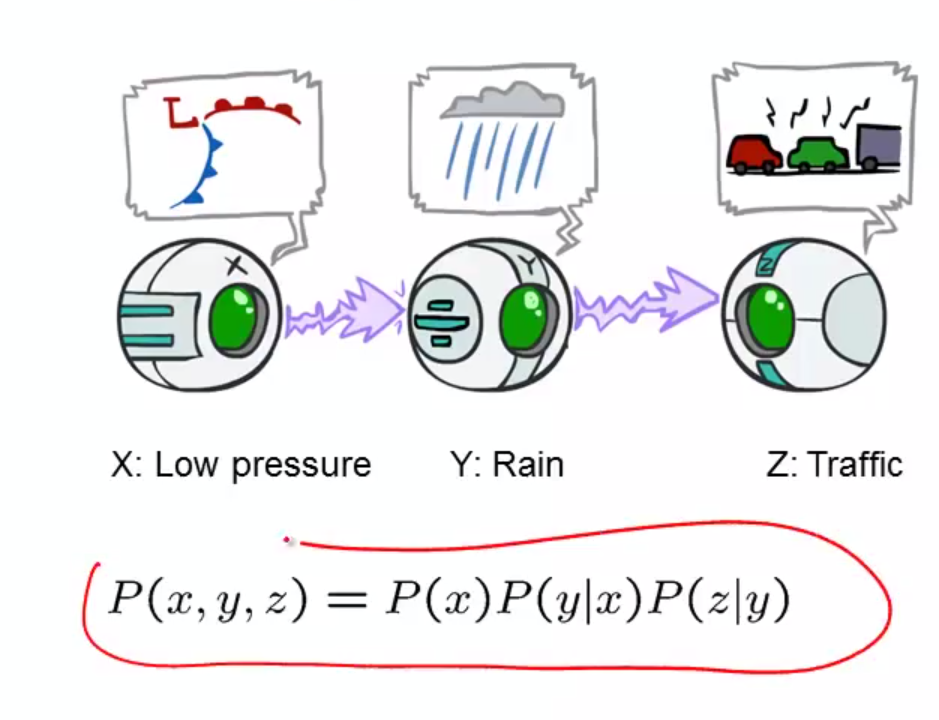
\includegraphics[scale=0.36]{snapshot128}
  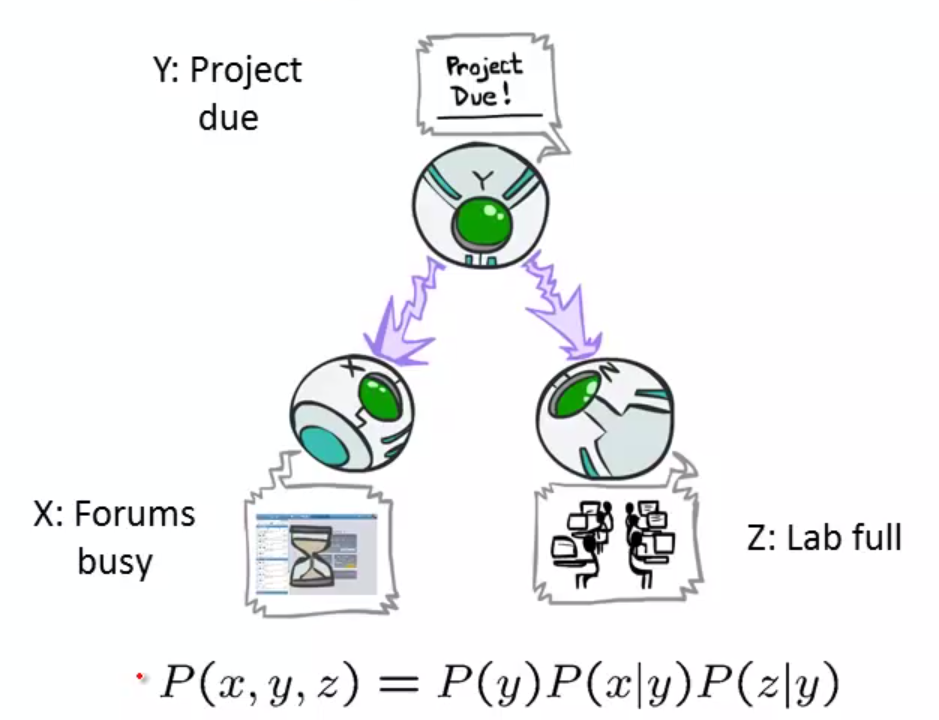
\includegraphics[scale=0.36]{snapshot127}
  \centering{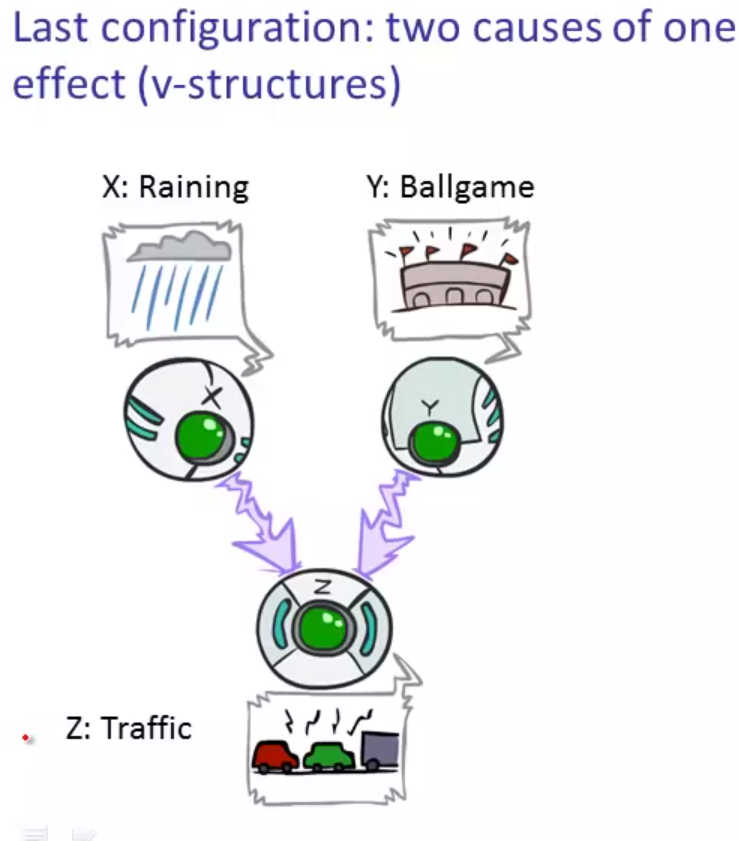
\includegraphics[scale=0.36]{snapshot129}}
\item \textbf{Reachability} Shade evidence nodes, look for paths in
  the resulting graph
\item Question: Are $X$ and $Y$ conditionally independent given
  evidence variable $Z$? \textbf{Yes}, if $X$ and $Y$ are
  ``d-separated'' by $Z$. How-to? Consider all undirected paths from
  $X$ to $Y$, if there is \textbf{no active paths}, we get (conditional)
  independence. Namely, if ALL paths are inactive, then the
  (conditional) independence is guaranteed.
\item All it takes to block a path is \textbf{a single INACTIVE}
  segment.
\item A Bayes Net's joint distribution may have further (conditional)
  independence that is not detectable until you inspect its specific
  distribution. 
\end{itemize}


\subsection{Bayes Nets: Inference}
\label{sec:bayes-nets:-infer}

\begin{itemize}
\item \textbf{Inference} Calculating some useful quantity from a joint
  probability distribution.
\item Core of this part is to find \textbf{more effective ways} to do
  ``inference by enumeration''.
\item \textbf{Variable Elimination} Interleave joining and
  marginalizing. 
\item Marginalization: Take a factor and sum out a variable. Aka it
  shrinks a factor to a smaller one; in Communication, they say it's a
  \textbf{projection} operation. (In math, they say let's do
  \textbf{differentiation}.) 
\item $A+\bar{A}=1$ and $A\cdot\bar{A}=0$
\item All we are doing is exploiting \textbf{math equations/tricks}
  to? Improve \textbf{computational efficiency}. So that rolls back to
  my good old question---What if we have a computer with infinite
  \textbf{computation power}? What would we do with that?
\item The computational and space complexity of variable elimination
  is determined by the largest factor.
\item If we can answer $P(z)$ equals to $0$ or not, we answered the
  3-SAT problem has a solution. Hence \textbf{inference} in Bayes Net
  is \textbf{NP-hard}. \textbf{No known efficient} probabilistic
  inference in general.
\item A polytree is a directed graph with \textbf{no undirected}
  cycles. 
\item Remember to pick the ordering of elimination that is EFFICIENT.
\end{itemize}

\subsection{Bayes Nets: Sampling}
\label{sec:bayes-nets:-sampling}

\begin{itemize}
\item 
\end{itemize}

\section{Learning}
\label{sec:learning}


\subsection{Reinforcement Learning 1}
\label{sec:reinf-learn-1}

\begin{itemize}
\item Basic idea:
  \begin{itemize}
  \item Receive feedback in the form of \textbf{rewards}
  \item Agent's utility is defined by the \textbf{reward function}
  \item Must (learn to) act so as to \textbf{maximize expected
      rewards}
  \item Rule of thumb: All learning is based on what? \textbf{Observed
    samples of outcomes}. Namely, sensing the elephant. When you take
  an action, you see what happens. But you \textbf{DO NOT} see
  everything that might happen.
  \end{itemize}
\item New twist: don't know Transition function or reward
  function. Must actually \textbf{try actions and states} out to
  learn. 
\item Offline (MDPs). Online (Reinforcement Learning). (And then
  pretend that it is true.)
\item \textbf{Model-Based Idea} Learn an approximate model based on
  experiences (namely, empirical crap). Solve for values \textbf{as
    if} the learned model \textbf{were} correct. (WHAT IF it is not
  correct? Then go fuck yourself.) This is, indeed how the
  state-of-the-art data mining, machine learning, and maybe cock
  sucking works.
\item Model-Based Learning: Learn the empirical MDP model, then solve
  the \textbf{learned} MDP.
\item $E[A]=\sum_{a}P(a)\cdot a$ This is $100\%$ valid when we
  \textbf{know} $P(A)$. Without $P(A)$, we can \textbf{try to} collect
  samples $[a_{1},a_{2},\ldots,a_{N}]$.
  \begin{itemize}
  \item For Model Based, we have $\hat{P}(a)=\dfrac{num(a)}{N}$
    Eventually you learn the right model.\\[1pt]
  \item For Model Free, we just do $E[A]\simeq \dfrac{1}{N}\sum_{i}
    a_{i}$ Samples appear with the \textbf{right frequencies}.
  \end{itemize}
\item Passive Reinforcement Learning: Goal is to learn the
  \textbf{state values} by inputting/carrying out a fixed policy
  (namely, action/signal).
\item We are missing something! But in the end, it's an average. It's
  an \textbf{average} of a bunch of things, each thing is a
  \textbf{one-step reward} plus a \textbf{discounted future} from
  \textbf{previous computation}. (Aren't math and natural language
  description sucking? Indeed they are.)
\item \textbf{Sample-Based Policy Evaluation} Take samples of outcomes
  $s'$ (by doing the ACTION!) and \textbf{average}.
\item Big Idea: Learn from every experience. Namely: Update $V(s)$
  each time we experience a transition $(s,a,s',r)$. How?
  $V^{\pi}\leftarrow (1-\alpha)V^{\pi}(s)+(\alpha)*sample$ The fucking
  $\alpha$ is called learning rate.
\item You can think of that as an
  \textbf{error}. $V^{\pi}(s)\leftarrow V^{\pi}(s)+\alpha (sample -
  V^{\pi}(s))$ Adjust your estimate in  the direction of error by some
  small step size of $\alpha$. In communication, they call the crap
  \textbf{Affine Projection} algorithm.
\item Running interpolation update: $\bar{x}_{n}=(1-\alpha)\cdot
  \bar{x}_{n-1}+\alpha\cdot x_{n}$
\item \textbf{Active Reinforcement Learning} {\color{red} learn the
    optimal policy/values}
\item But Q-Values are \textbf{more useful} (how the heck do you know
  that it is more useful? By trials and errors indeed.)
\item
  $Q_{k+1}(s,a)\leftarrow\sum_{s'}T(s,a,s')[R(s,a,s')+\gamma\displaystyle{\max_{a'}}Q_{k}(s',a')]$
  This crap is called sample-based Q-value recursion/iteration. Key
  idea: instead of looking at \textbf{two consecutive} {\color{red}
    values}, let us look at \textbf{two consecutive}
  Q-values. (Namely, because they are ``more useful''. Practically,
  they are relatively easy to, you guessed it, COMPUTE.)
\item Q-Learning converges to \textbf{optimal} policy, even if you are
  acting \textbf{suboptimally}! Caveats:
  \begin{itemize}
  \item You have to explore enough.
  \item You have to eventually make the learning rate small enough.
  \item Basically, in the limit, it doesn't matter how you select
    actions. (Note: In the end, you will learn that cliff jumping is
    bad.)
  \end{itemize}
\end{itemize}

\subsection{Reinforcement Learning 2}
\label{sec:reinf-learn-2}

\begin{itemize}
\item \textbf{Big idea} Compute all averages over $T$ using sample
  outcomes, namely by trials and errors.
\item The problem is, that I \textbf{do not} know the transition
  function.
\item \textbf{Exploration} You try things, which may be
  disasters. Namely, you just do not know the \textbf{pits} until you
  try it.
\item \textbf{Exploitation} You do the things which currently appear
  to be good.
\item How to explore? Simplest, random actions
  ($\epsilon$-greedy). Possible solution to problems: lower $\epsilon$
  over time; use exploration functions.
\item One sample exploration function is: take a value estimate $u$
  and a visit count $n$, returns an optimistic utility:
  $f(u,n)=u+k/n$. ``You try things that are known to lead to things
  that are unknown.''
\item \textbf{Regret} is a measure of your total mistake cost: the
  difference (namely, do a comparison or subtraction or
  differentiation, whatsoever you like.) between your
  expected rewards, including youthful suboptimality, AND
  optimal (expected) rewards.
\item Minimizing regret goes beyond learning to be optimal---it
  requires \textbf{optimally learning to be optimal}. (Comment:
  Regret, balabala, value iteration all such and such are fancy names
  given by \textbf{Computer Scientists} to ease the fear of dealing
  with TONS of mathematical equations. Namely, to concrete those
  fucking math abstractions---equations, inequations.) All in all,
  these are the ABSTRACTIONS (simulation, modeling, whatsoever) of our
  WORLD.   
\item Anyway, those models do work, under certain circumstances. 
\item Instead and In reality we want to \textbf{generalize}:
  \begin{itemize}
  \item Learn about some small number of training states from
    experience (or part of the real states, namely, test states)
  \item Generalize that experience to new, similar situations
  \item This is a fundamental idea in \textbf{machine learning},
    namely, build a MODEL or heuristic, and see if it works.
  \end{itemize}
\item You are going to learn faster if you do not have to
  \textbf{repeat} lessons in every \textbf{similar state}.
\item \textbf{Features} are functions from states to real numbers
  (often 0/1) that capture \textbf{important} properties (namely,
  CORRECTLY describes) of the state.
\item ``Give me a transition so that I can learn.''
\item ``You compute how wrong you were, and you try to make that
  number less.''
\item Adjust \textbf{weights} of active features.
\item Q-learning priority: Get Q-values close (modeling). Action
  selection priority: get ordering of Q-values right
  (prediction). Solution: learn policies that maximize
  \textbf{rewards}, not the value that predict them. Namely, care more
  about PREDICTION. More namely, care more about, well, you named it,
  ``FUTURE''.
\item Better methods exploit lookahead structure, sample wisely,
  change parameters\ldots
\end{itemize}
\end{document}

%%% Local Variables:
%%% mode: latex
%%% TeX-master: t
%%% End:
